\section{Introduction}
\label{sec:intro}

In recent years, Transformer~\cite{vaswani2017attention} has become a \textit{de facto} standard model architecture in Natural Language Processing~\cite{brown2020language,devlin2018bert,liu2019roberta},
and it is becoming common in many domains including Computer Vision~\cite{dosovitskiy2020image,liu2021swin,touvron2021training} and Speech Recognition~\cite{baevski2020wav2vec,chen2021wavlm,hsu2021hubert}.
However, efficient deployment of Transformer architectures has been challenging due to their large model size and high inference latency.
As a promising way to tackle this challenge, structured pruning of Transformers has been widely studied.

While prior work on pruning Transformers substantially reduces the inference time, it is often difficult to use in practice for several reasons.
First, previous approaches require retraining the pruned model and/or jointly learning the pruning configurations during training.
This increases the training time by up to 10$\times$~\cite{lagunas2021block, xia2022structured}, adding significant computational overhead.
Second, previous methods add many moving parts to the model deployment process.
That is, the pruning pipelines are often complex and require additional hyperparameter tuning.
Such techniques demand significant engineering efforts for implementation and debugging, which impedes their adoption in production pipelines.
Third, these previous methods do not directly adapt to the users' constraints.
They either rely on vague regularization hyperparameters to control the model sparsity or use fixed model architectures selected independently of the user settings.
This can result in sub-optimally pruned models that are not tailored to the users' constraints and hardware.

%%%%%%%%%%%%%%%%%%%%%%%%%%%%%%%%%%%%%%%%%%%%%%%%%%%%%
\begin{figure}[t]
\centering
    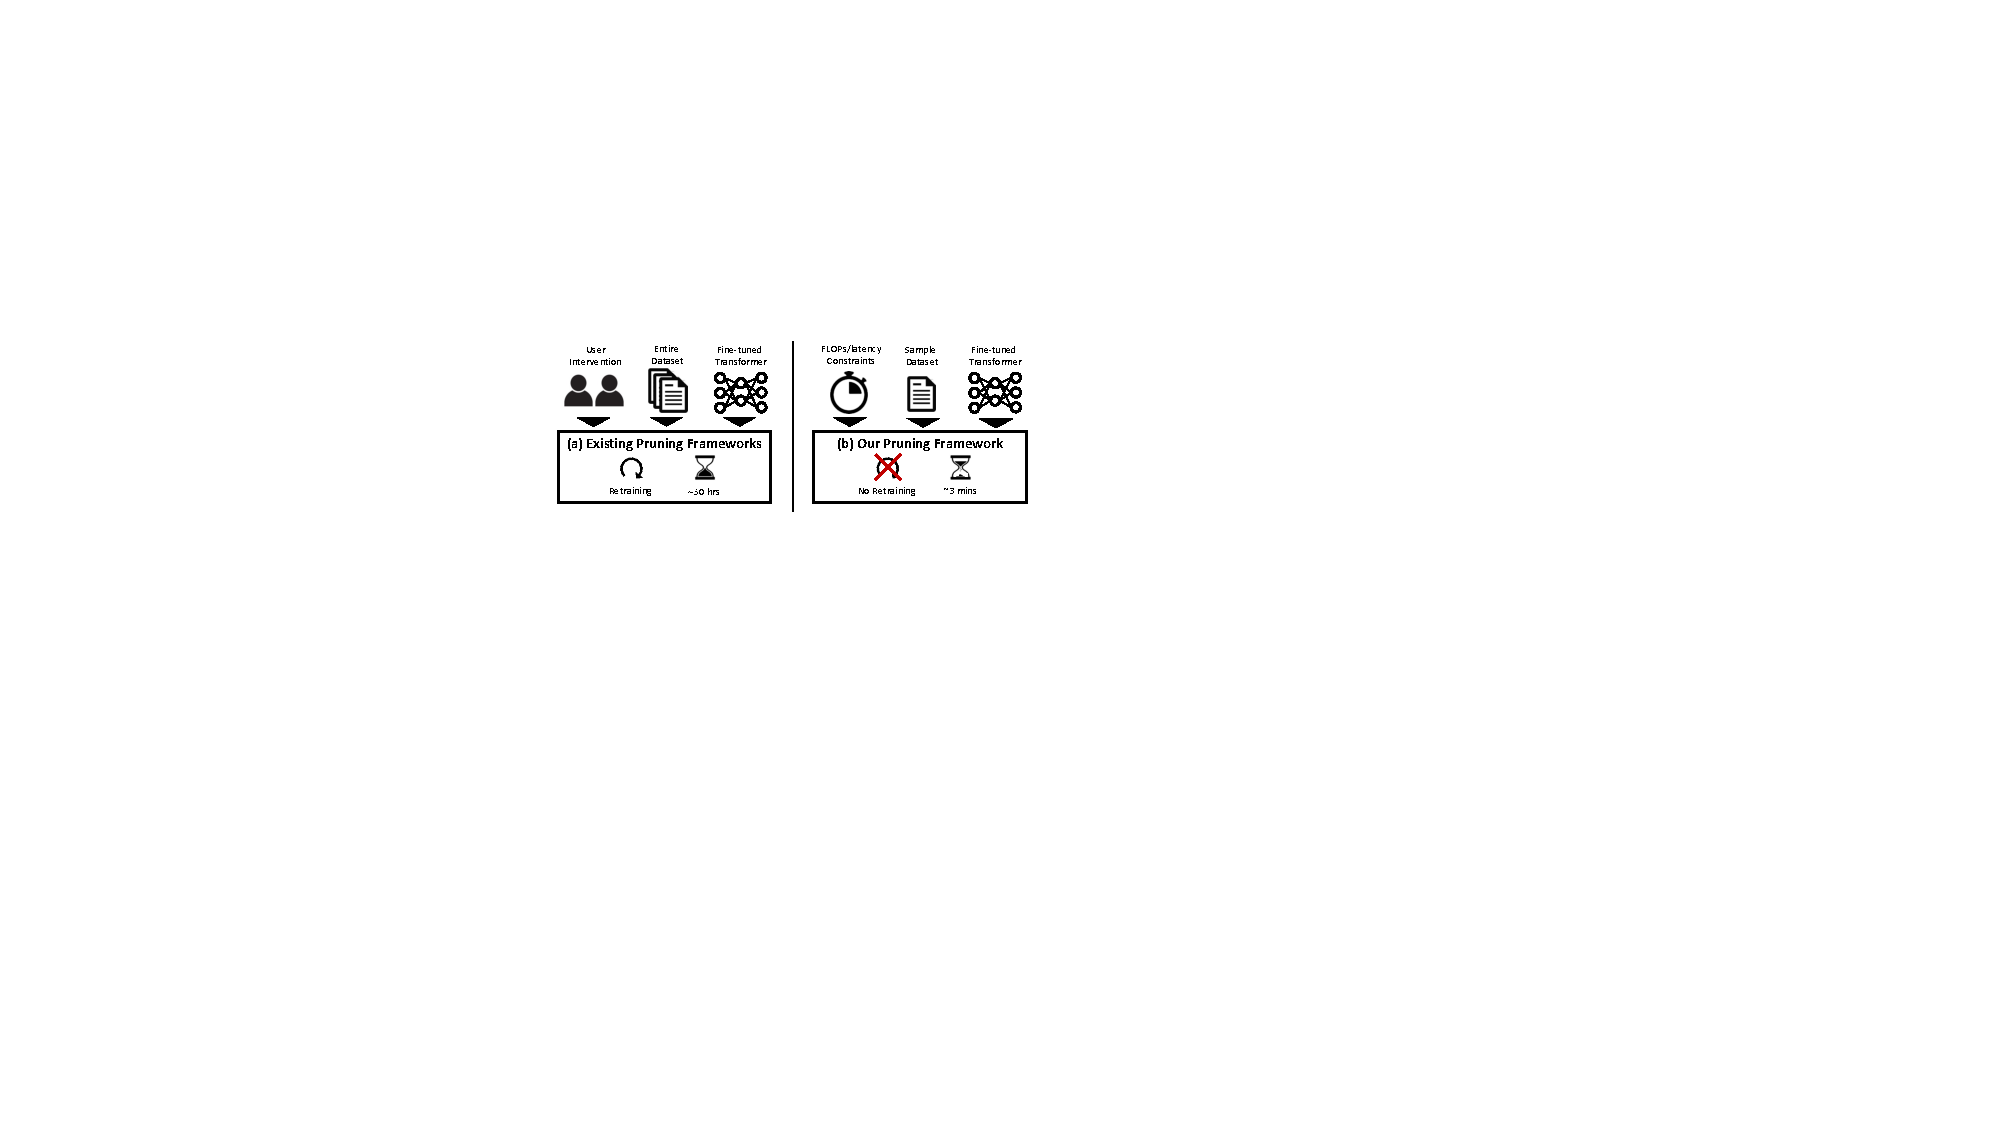
\includegraphics[width=0.8\textwidth]{figures/overview.pdf}
\caption{
(a) Prior pruning frameworks require additional training on the entire training set and involve user intervention for hyperparameter tuning.
This complicates the pruning process and requires a large amount of time (e.g., $\sim$30 hours).
(b) Our pruning framework does not require retraining. 
It outputs pruned Transformer models satisfying the FLOPs/latency constraints within considerably less time (e.g., $\sim$3 minutes), without user intervention.
}
\vspace{-5mm}
\label{fig:overview}
\end{figure}
%%%%%%%%%%%%%%%%%%%%%%%%%%%%%%%%%%%%%%%%%%%%%%%%%%%%%

To address the above limitations, we propose a fast \textit{post-training pruning} framework for Transformers that does not require any retraining of the models.
As illustrated in \fref{fig:overview}, our framework takes as input a Transformer model, a sample dataset, and a FLOPs/latency constraint.
It then outputs a pruned Transformer model that can be deployed immediately.
By avoiding expensive retraining, the end-to-end pruning pipeline can be extremely fast and simplified, which typically takes a few minutes without any user interventions that complicate the whole process.

Indeed, post-training compression has been widely studied for quantization, and it gained considerable attention in both academia and industry~\cite{banner2018post,hubara2020improving,zhao2019improving}. 
Although quantization-aware training methods
%that perform retraining during or after quantization
achieve higher compression rates in general, post-training quantization (PTQ) has often been more preferred in practice due to its retraining-free advantages.
Importantly, PTQ allows quantization to happen seamlessly at the model deployment time using the tools such as TensorRT~\cite{tensorrt}, TFLite~\cite{tflite}, and OpenVINO~\cite{openvino}.
Similar to the PTQ methods, our framework provides an out-of-the-box tool that enables pruning of Transformers without engineering~efforts.

Our contributions can be summarized as follow:
\vspace{-2mm}
\begin{itemize}[leftmargin=*]
    \item We propose a novel post-training pruning framework for Transformers that does not require model retraining.
    To retain accuracy without retraining, our framework consists of three stages:
    (i) the \textit{mask search} process guided by the Fisher information matrix to select which heads/filters to prune (\sref{subsec:search});
    (ii) the \textit{mask rearrangement} process that reselects the heads/filters to prune by capturing intra-layer interactions (\sref{subsec:rearrange});
    and (iii) the \textit{mask tuning }process that adjusts the mask variables to ensure that the output signal is recovered for each layer (\sref{subsec:tuning}).
    
    \item We extensively test our framework by applying it to BERT$_\textsc{base}$ and DistilBERT on GLUE and SQuAD tasks (\sref{subsection:performance}).
    Within 1$\%$ of accuracy drop, our framework reduces 30--50$\%$ of the original FLOPs (\fref{fig:flops_result}), resulting in up to 1.56$\times$ speedup on an NVIDIA V100 GPU (\tref{tab:latency_result}).
    \item We show that our method achieves comparable or even better FLOPs-accuracy trade-off than prior structured pruning methods \textit{without} retraining (\sref{subsection:comparison}, \fref{fig:comparison}).
    Our end-to-end pruning pipeline finishes in only 39 and 135 seconds on average for GLUE and SQuAD (\sref{subsection:analysis}, \tref{tab:time_breakdown}), which is over 100$\times$ faster than the retraining-based methods.
\end{itemize}
